\documentclass[a4paper,12pt,oneside,openany,table,xcdraw]{article}

\usepackage{setspace}
\usepackage{multirow}
\usepackage{hyperref}
\usepackage{caption}
\usepackage{indentfirst}
\usepackage{tikz} %% fasores
\usetikzlibrary{arrows,arrows.meta,quotes,angles}
\usepackage{siunitx}

\usepackage[brazilian]{babel}
\usepackage[utf8x]{inputenc}
\usepackage{amsmath, graphicx, subfig, enumerate}
\usepackage{float, verbatim}
\usepackage[colorinlistoftodos]{todonotes}
\usepackage{makeidx}
\usepackage{geometry}

\graphicspath{{img/}}
\geometry{a4paper, hmargin={3cm, 3cm}, vmargin={3cm, 2cm} }
\setlength{\parindent}{1.0cm}
\captionsetup{font=small}

\begin{document}
\newcommand{\thedepartment}{Faculdade de Engenharia Elétrica}
\newcommand{\thecourse}{FEELT}
\newcommand{\thetitle}{VERIFICAÇÃO DA SEQUÊNCIA DE FASES DAS TENSÕES}
\newcommand{\thetype}{Relatório da Disciplina de Experimental de Circuitos Elétricos II}
\newcommand{\theproftitle}{Bacharel em Engenharia Elétrica}
\newcommand{\thestudent}{Lesly Viviane Montúfar Berrios\\
\centering11811ETE001}
\newcommand{\theadvisor}{Prof. Wellington Maycon Santos Bernardes}
\newcommand{\thecity}{Uberlândia}

\thispagestyle{empty}\newcommand*{\themonth}{\ifthenelse{\the\month < 2}{Janeiro }
                  {\ifthenelse{\the\month < 3}{Fevereiro }
                  {\ifthenelse{\the\month < 4}{Março }
                  {\ifthenelse{\the\month < 5}{Abril }
                  {\ifthenelse{\the\month < 6}{Maio }
                  {\ifthenelse{\the\month < 7}{Junho }
                  {\ifthenelse{\the\month < 8}{Julho }
                  {\ifthenelse{\the\month < 9}{Agosto }
                  {\ifthenelse{\the\month < 10}{Setembro }
                  {\ifthenelse{\the\month < 11}{Outubro }
                  {\ifthenelse{\the\month < 12}{Novembro }{Dezembro }}}}}}}}}}}}
                  
\begin{titlepage}
\begin{center}

	\vspace{-0.5cm}

  \begin{figure}[hbt!]
		\begin{center}
		   
\includegraphics[width=2.8cm]{ufu-logo.png}
		\end{center}
	\end{figure}
 	%\vspace{-4cm}

%\begin{doublespacing}

  \Large{\textbf{Universidade Federal de Uberlândia}}\\
  \large{\thedepartment}\\
  \large{\thecourse}\\


\vspace{5.8cm}
  \par
  \large\textbf{\thetitle}
\vspace{5.8cm} 

%\end{doublespacing}
  \par
  \thetype\\
  por\\
  %\hspace{2cm}\large{}\\

\vspace{0.8cm}
\par
  \normalsize{\thestudent}\\ [2cm]
  \theadvisor

\par\vfill
  \thecity, \themonth / \the\year

\end{center}

\end{titlepage}

%% Comeca o documento !

\onehalfspacing
\tableofcontents % sumário
\newpage

\section{Objetivos} % 2,5%
Pretende-se verificar experimentalmente conceitos teóricos de como encontrar a correta sequência de
fase diante da ausência de um sequencímetro (método do voltímetro).

\section{Introdução teórica} % 5%

O sequencímetro é um instrumento de medida elétrica analógica ou digital que tem por  finalidade a verificação da sequência de fases de um motor trifásico (circuito alimentado por corrente alternada), ou seja, indica a fase aberta e o sentido de rotação do motor. Na Figura \ref{intro:fig1}, é observado um fasímetro, que possui a mesma função, havendo poucas diferenças, entre elas, estão a tensão de entrada e a faixa de frequência. Sobre seu funcionamento diz-se que, a partir do momento em que o sequencímetro detecta a passagem por zero (pulso positivo de curta duração) de cada fase é aplicado em um circuito sequencial feito com flip-flop e indica a sequência da rede \cite{UNIR}.

Na ausência desse tipo de equipamento, circuitos desequilibrados podem ser utilizados para a verificação de sequência de fases em certo sistema elétrico. Basendo-se na queda de tensão em cada fase, é possível provar matematicamente qual é a sequência de fases utilizada, conforme a Sessão \ref{m1:teorico}.

\vspace{0.5cm}
\begin{figure}[H]
\centering
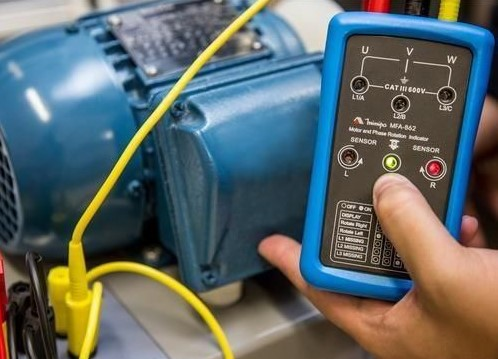
\includegraphics[width=12.5cm]{fasimetro}
\caption{Fasímetro com indicador led 690 volts - MFA-862 \cite{fig1}.}
\label{intro:fig1}
\end{figure}
\vspace{0.3cm}


\section{Preparação}
\subsection{Materiais e ferramentas} % 2,5%
\begin{enumerate}[1 -]
\item \emph{\textbf{Fonte:}}
Alimentará todo o circuito. Possui frequência de $60\ Hz$.

\item \emph{\textbf{Regulador de tensão (Varivolt):}}
Também chamado de autotransformador, permitirá obter o valor desejado de corrente a partir da regulagem correta da tensão fornecida pela fonte.

\item \emph{\textbf{Conectores:}}
Para as conexões no circuito foi utilizado majoritariamente cabos banana-banana.

\item \emph{\textbf{Medidor eletrônico KRON Mult K:}}
Possibilita encontrar a medição da potência real (P) - vatímetro, reativa (Q) e aparente (S) do circuito. Ele também possui função de cofasímetro, instrumento elétrico que mede o fator de potência (fp, $cos\theta$) ou o ângulo da impedância $\theta$ do circuito, para um circuito com a impedância $Z = Z\angle \theta$.

\item \emph{\textbf{Amperímetro analógico AC:}}
Instrumento utilizado para acompanhar visualmente o aumento da corrente.

\item \emph{\textbf{Resistor de $50\Omega$:}}
Carga resistiva para compor a carga do circuito trifásico.

\item \emph{\textbf{Capacitor de $45,9\mu F$:}}
Sendo sua resistência quase nula, portanto desprezível nessa aplicação (Esquenta pouco, logo dissipa menos energia).
\end{enumerate}

\vspace{0.2cm}
\subsection{Montagem} % 2,5%

\subsubsection{Verificação da sequência de fases}
A montagem para o método do voltímetro pode ser realizado por meio de voltímetros analógicos, como mostra a Figura \ref{m1:analogico}, ou mediante equipamento digital, como na Figura \ref{m1:esquema}. Para este experimento utilizou o medidor digital \emph{Kron}, com configuração TL=0000 (Trifásico Equilibrado ou Desequilibrado Estrela - 3F + N - 3 elementos 4 fios). 
Assim, no caso de equipamento digital, aplica-se uma tensão linha $V_L=100V$ com o auxílio do \emph{Varivolt}, em frequência de 60Hz, e parâmetros de carga: $R=50\Omega$ e $C=45,9 \mu F$. Ademais, como procedimento de segurança, é verificado sempre se existe algum curto-circuito em alguma das fases em baixa tensão.

\vspace{0.2cm}
\begin{figure}[H]
\centering
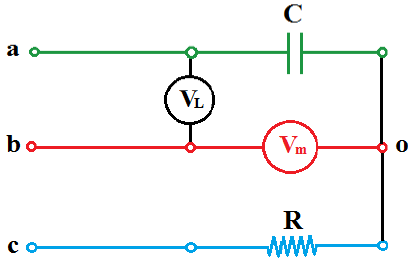
\includegraphics[width=11.5cm]{m-analog}
\caption{Método do voltímetro, utilizando-se voltímetros analógicos.}
\label{m1:analogico}
\end{figure}

\vspace{0.3cm}
\begin{figure}[H]
\centering
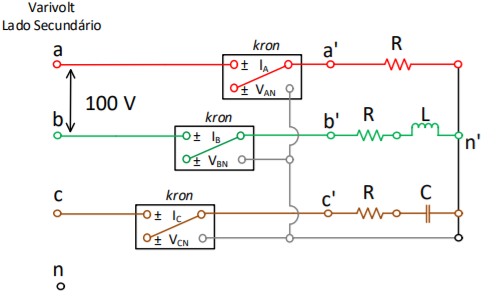
\includegraphics[width=13cm]{m1-circuito}
\caption{Método do voltímetro, utilizando-se equipamento digital.}
\label{m1:esquema}
\end{figure}
\vspace{0.1cm}

\subsubsection{Verificação da sequência de fases - Fase A aberta}

\subsubsection{Verificação da sequência de fases - Fase C aberta}



\section{Dados Experimentais}
Embora, esta sessão seja reservada para os dados obtidos experimentalmente, também são comptemplados, nas tabelas que seguem, os resultados teóricos.

\subsubsection{Verificação da sequência de fases}


\subsubsection{Verificação da sequência de fases - Fase A aberta}

\subsubsection{Verificação da sequência de fases - Fase C aberta}




\section{Análise sobre segurança} % 2,5%
Os óculos de segurança são Equipamentos de Proteção Individual (EPIs) e são utilizados para a proteção da área ao redor dos olhos contra qualquer tipo de detrito estranho, que possa causar irritação ou ferimentos. Também protegem contra faíscas, respingos de produtos químicos, detritos, poeira, radiação e etc \cite{safe}.
É importante a utilização desse equipamento durante os experimentos a fim de evitar qualquer dano, além de preparar o profissional para o manejo correto e seguro de qualquer equipamento.
Além disso, foi de extrema importância a presença do professor ou técnico na verificação da montagem do circuito antes de energizá-lo. Assim, reduziu-se riscos de curtos-circuitos ou sobrecarga na rede.


\section{Cálculos, análise dos resultados e questões} % (quando houver) (70%)
\subsection{Análise teórica do circuito} \label{m1:teorico}
\subsubsection{Verificação da sequência de fases}

\subsubsection{Verificação da sequência de fases - Fase A aberta}

\subsubsection{Verificação da sequência de fases - Fase C aberta}

\subsection{Reflexão}
\subsubsection{E na ausência de um voltímetro?}
% - Na impossibilidade de ter voltímetros, amperímetros e sequencímetro, como você poderia encontrar a solução desse problema (abc ou cba)?
 Na ausência de voltímetros, amperímetros ou sequencímetro, pode-se utilizar equipamentos permitam de forma visual ou sensitiva identificar a fase com maior e maior tensão, para assim prosseguir com a análise realizada neste experimento. 

\subsubsection{Sobre a importância da sequência de fase em um circuito elétrico}
% - Aponte a importância de encontrar a correta sequência de fase em um circuito elétrico.


\newpage
\section{Simulação computacional} % (10%);
Para a simulação foi utilizada uma fonte CBA, por isso pode haver alguma estranheza no circuito por parte do leitor. No entanto, a análise é a mesma.
\vspace{0.2cm}

\subsubsection{Verificação da sequência de fases}

\begin{figure}[H]
\centering
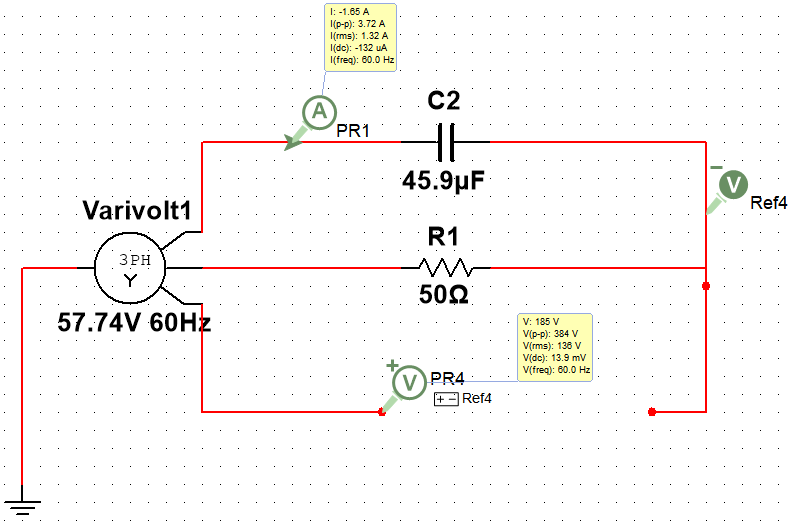
\includegraphics[width=13cm]{m1-sim-abc}
\caption{Método do voltímetro, utilizando-se equipamento digital.}
\label{m1:sim:abc}
\end{figure}

\vspace{0.2cm}
\begin{figure}[H]
\centering
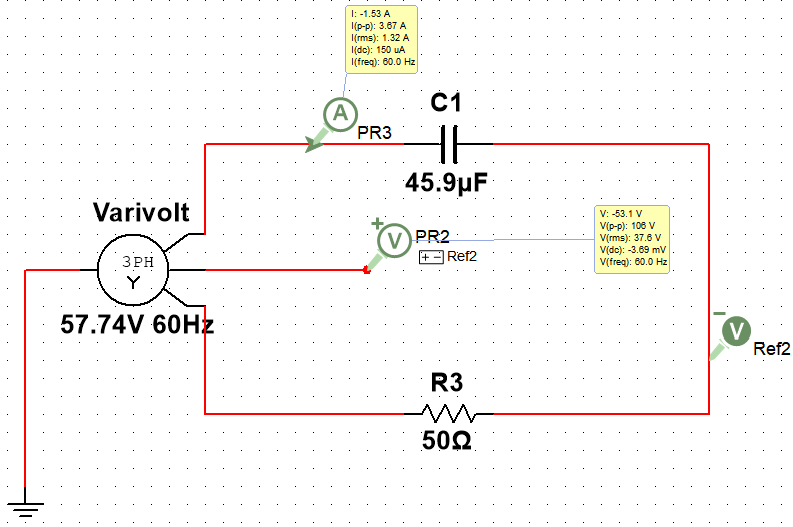
\includegraphics[width=13cm]{m1-sim-cba}
\caption{Simulação para determinação de sequência de fase CBA.}
\label{m1:sim:cba}
\end{figure}

\subsubsection{Verificação da sequência de fases - Fase A aberta}
\begin{figure}[H]
\centering
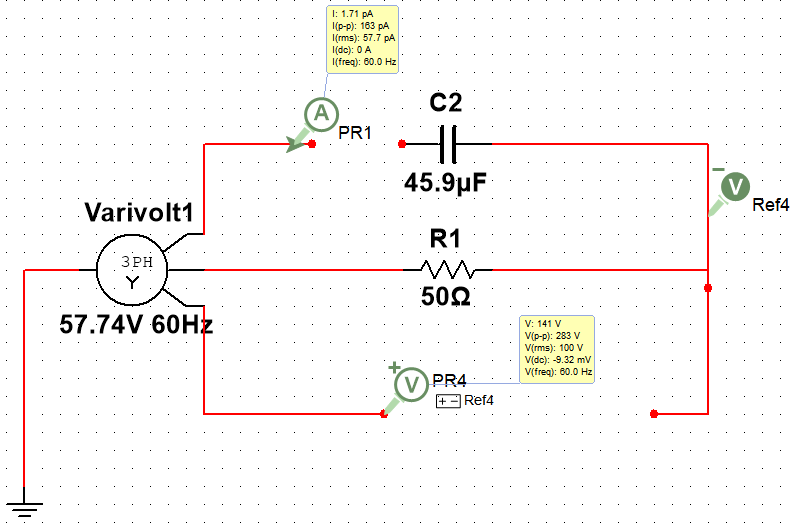
\includegraphics[width=13cm]{m2-sim-abc}
\caption{Método do voltímetro, utilizando-se equipamento digital.}
\label{m2:sim:abc}
\end{figure}

\vspace{0.2cm}
\begin{figure}[H]
\centering
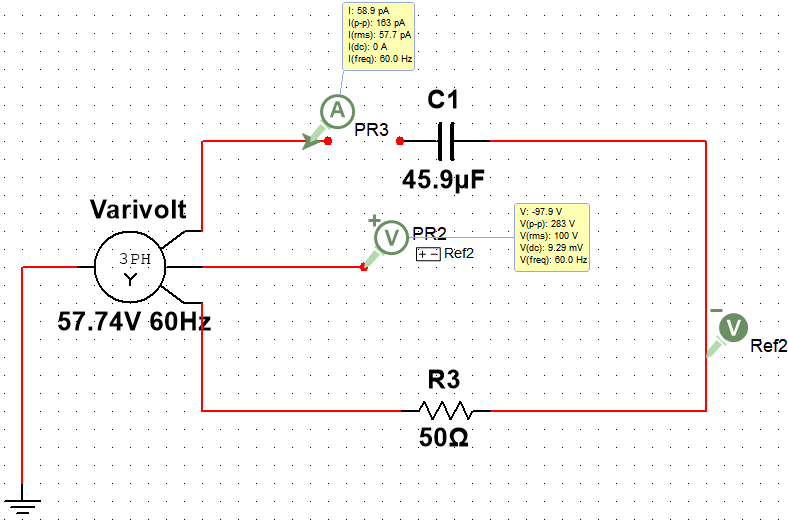
\includegraphics[width=13cm]{m2-sim-cba}
\caption{Simulação para determinação de sequência de fase CBA.}
\label{m2:sim:cba}
\end{figure}

\subsubsection{Verificação da sequência de fases - Fase C aberta}
\begin{figure}[H]
\centering
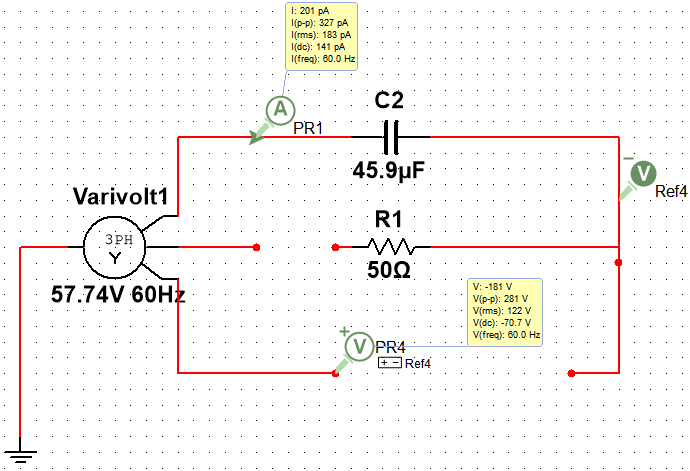
\includegraphics[width=13cm]{m3-sim-abc}
\caption{Método do voltímetro, utilizando-se equipamento digital.}
\label{m3:sim:abc}
\end{figure}

\vspace{0.2cm}
\begin{figure}[H]
\centering
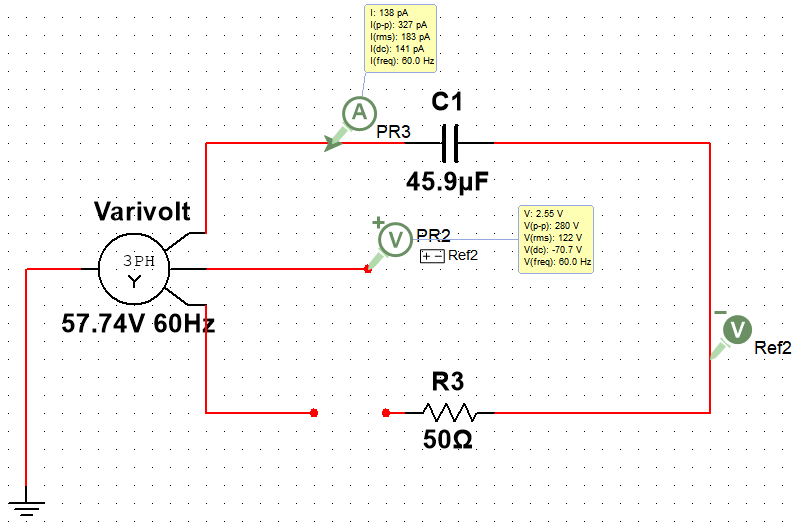
\includegraphics[width=13cm]{m3-sim-cba}
\caption{Simulação para determinação de sequência de fase CBA.}
\label{m3:sim:cba}
\end{figure}

\newpage
\section{Conclusões} % (no mínimo 10 linhas) (5%);


\newpage
\begin{thebibliography}{9} 
% Introdução
\bibitem{PH}
    P. H. O. Rezende,
    "Circuitos Polifásicos Desequilibrados", 2018.

\bibitem{safe}
    SafetyTrabi,
    “Óculos de segurança: Saiba quando utilizar este EPI”, SafetyTrab, 2019.
 Disponível em:
 \url{https://www.safetytrab.com.br/blog/oculos-de-seguranca/}. Acesso em: ago. 2019.

\bibitem{UNIR}
    B. M. Nascimento, J. Carneiro, P. Viecilli,
    “Sequencímetro de Baixo Custo”, Fundação Universidade Federal de Rondônia - UNIR.
 Disponível em:
 \url{https://brunomarquesunir.wixsite.com/sequencimetro}. Acesso em: dez. 2019.

\bibitem{fig1}
    Dutra Máquinas.
 Disponível em:
 \url{https://m.dutramaquinas.com.br/p/fasimetro-com-indicador-led-690-volts-mfa-862-mfa-862}. Acesso em: dez. 2019.


\end{thebibliography}
\end{document}
